\documentclass[12pt,a4paper]{article}
\usepackage[utf8]{vietnam} % Gõ tiếng Việt
\usepackage{amsmath,amssymb} % Gõ công thức toán
\usepackage[top=2.5cm,bottom=2.5cm,left=2.5cm,right=2.5cm]{geometry} % Căn lề
%=====Tạo tiêu đề trên và dưới====%
\usepackage{fancyhdr}
\pagestyle{fancy}
\fancyhf{}
\renewcommand{\headrulewidth}{0.5pt}
\renewcommand{\footrulewidth}{0.5pt}
\lhead{Biên soạn: TS. Nguyễn Kiều Linh}
\rhead{Học viện Công nghệ Bưu chính Viễn thông}
\lfoot{Số điện thoại 0985059646}
\fancyfoot[R]{Trang \thepage}
%=====EndTạo tiêu đề trên và dưới====%
\usepackage[loigiai]{ex_test} % dethi
\renewtheorem{ex}{\color{blue} Câu}
\begin{document}
\Opensolutionfile{ans}[filedapan]
\begin{center}
{\bf\Large BÀI TẬP TOÁN RỜI RẠC 2}
\end{center}
\begin{ex}
Đồ thị bên dưới có mấy đỉnh trụ?
\begin{center}
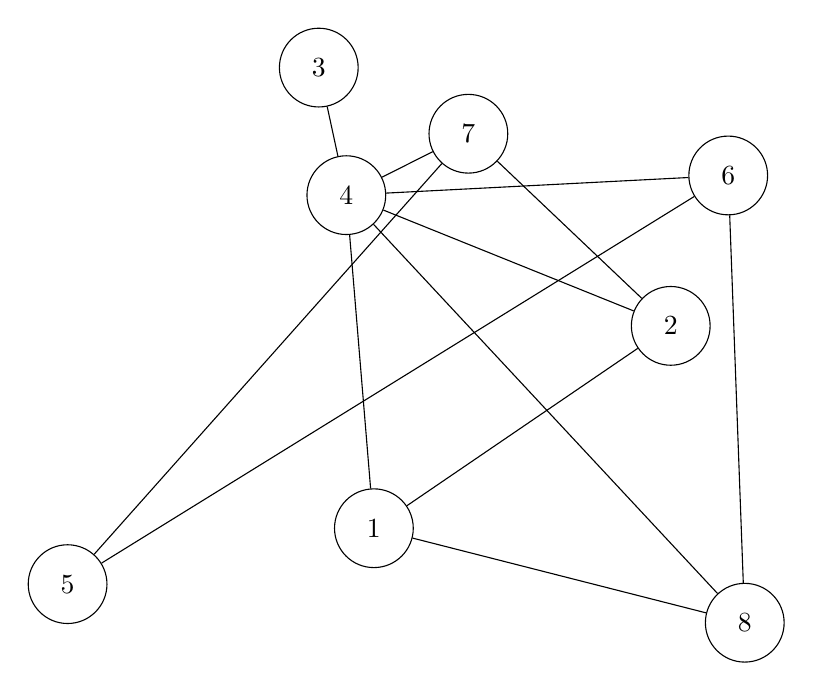
\begin{tikzpicture}[node distance=2cm, every node/.style={circle, draw, minimum size=1cm}]
  \node (1) at (-0.21, -2.28) {1};
  \node (2) at (3.56, 0.29) {2};
  \node (3) at (-0.91, 3.57) {3};
  \node (4) at (-0.56, 1.95) {4};
  \node (5) at (-4.10, -2.99) {5};
  \node (6) at (4.29, 2.20) {6};
  \node (7) at (0.99, 2.73) {7};
  \node (8) at (4.50, -3.48) {8};
  \draw (7) -- (4);
  \draw (2) -- (4);
  \draw (1) -- (2);
  \draw (8) -- (4);
  \draw (2) -- (7);
  \draw (8) -- (1);
  \draw (4) -- (3);
  \draw (6) -- (8);
  \draw (4) -- (6);
  \draw (5) -- (6);
  \draw (7) -- (5);
  \draw (4) -- (1);
\end{tikzpicture}
\end{center}

\choice
{1}
{4}
{\True 1}
{8}
\loigiai{}
\end{ex}

\begin{ex}
Đồ thị bên dưới có mấy cạnh cầu?
\begin{center}
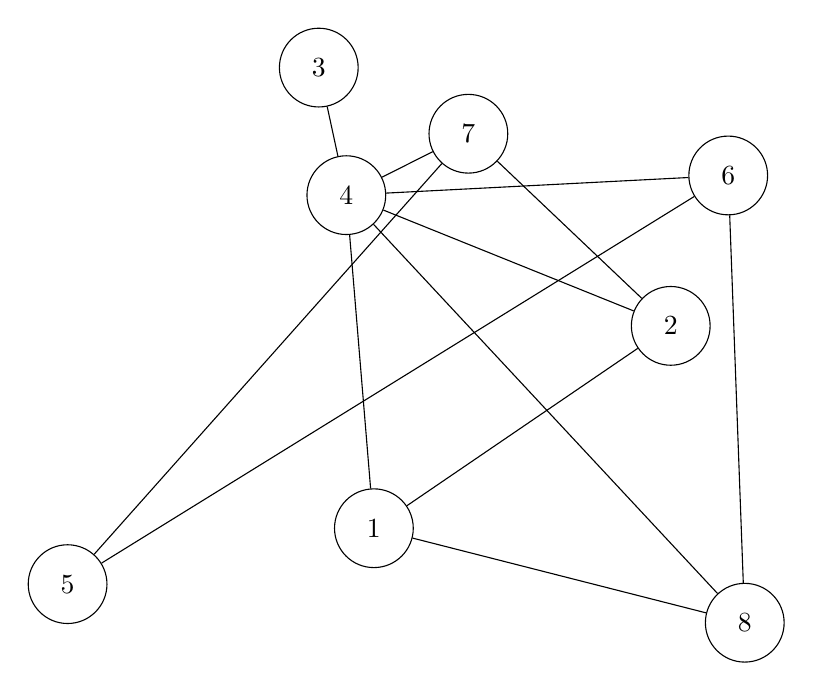
\begin{tikzpicture}[node distance=2cm, every node/.style={circle, draw, minimum size=1cm}]
  \node (1) at (-0.21, -2.28) {1};
  \node (2) at (3.56, 0.29) {2};
  \node (3) at (-0.91, 3.57) {3};
  \node (4) at (-0.56, 1.95) {4};
  \node (5) at (-4.10, -2.99) {5};
  \node (6) at (4.29, 2.20) {6};
  \node (7) at (0.99, 2.73) {7};
  \node (8) at (4.50, -3.48) {8};
  \draw (7) -- (4);
  \draw (2) -- (4);
  \draw (1) -- (2);
  \draw (8) -- (4);
  \draw (2) -- (7);
  \draw (8) -- (1);
  \draw (4) -- (3);
  \draw (6) -- (8);
  \draw (4) -- (6);
  \draw (5) -- (6);
  \draw (7) -- (5);
  \draw (4) -- (1);
\end{tikzpicture}
\end{center}

\choice
{7}
{2}
{5}
{\True 1}
\loigiai{}
\end{ex}
\Closesolutionfile{ans}
\end{document}